\section{Model}
\label{sec:model}

\setlength{\tabcolsep}{2pt}
\begin{figure*}
\begin{center}
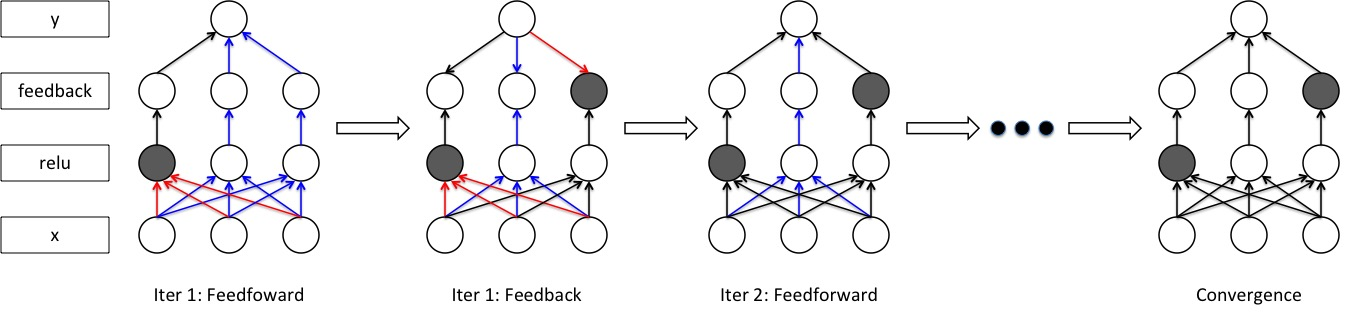
\includegraphics[width=0.95\linewidth]{figs/model/model}
% \vspace{-10pt}
\caption{Illustration of our feedback model and its inference process. At the first iteration, the model performs as a feedforward neural net. Then given the top signal neuron, the hidden layers update their gates to maximize the confidence for the top neuron. This process continues until convergence.}
\label{fig:visual_compare}
% \vspace{-30pt}
\end{center}
\end{figure*}

We first review the current state-of-the-art feedforward convolutional neural network architecture and then propose our feedback model on top of that. 

\subsection{Review of Feedforward Convolutional Neural Networks}
Deep convolutional neural networks (CNNs) with rectified linear unit (ReLU) and max-pooling layers have become the state-of-the-art in computer vision. These architectures consist of many stacked feedforward layers, Low-level stages tend to learn biologically plausible feature detectors, such as Gabor filters [14]. Detectors in higher layers learn to respond to concrete visual objects or their parts, e.g., [15].

In this work we use the Maxout networks [7], combined with dropout [21]. 

Maxout networks represent the state-of-the-art for object recognition in various tasks and have only been outperformed (by a small margin) by averaging committees of several convolutional neural networks. 
A similar approach, which does not reduce dimensionality in favor of sparsity in the representation has also been recently presented [22]. 

\textbf{Convolutional Layer:} The input to this layer can be an image or the output of a previous layer, consiting of $C$ input maps of width $M$ and height $N$: $x \in R_{M \times N \times C}$
\begin{equation}
y_l(i,j,c) = \sum_{u,v \in \mathcal{N}}\sum_{c'} w_{l}(u,v) \cdot y_{l-1}(i+u, j+v, c')
\end{equation}

\textbf{ReLU Layer:}
A ReLU layer is used to add the nonlinearity for the network. The operation is element-wise
\begin{equation}
y_l(i,j,c) = \max (0,y_{l-1}(i,j,c))
\end{equation} 

\textbf{Max-Pooling Layer:}
A max-pooling layer is used to reduce the dimensionality of the output from a convolutional layer as well as keep the translation invarianceproperty of a network for modeling deformable parts and objects at various image locations. The operation of a max-pooling layer is very similar to convolution, except  
\begin{equation}
y_l(i,j,c) = \max_{u,v \in \mathcal{N}} y_{l-1}(i+u, j+v, c)
\end{equation}

\textbf{Fully Connnected Layer:}
Finally, a few fully connected layers (normally with drop-out) is stacked on top of the convolutional outputs to compute the scores of every class. 
\begin{equation}
\vec{y}_l = W_l^T  \vec{y}_{l-1}
\end{equation}

\subsection{Reinterpret ReLU and Max-Pooling Layer}
We model the max function as neuron activation gates $h$ with binary values 0 or 1. For the ReLU layer, the gates work as turn on the neuron to let the below message pass or turn off the neuron to stop the message flow. For the Max-Pooling layer, the gates work similarly as ReLU, except only one gate can be open among a local region.

For the ReLU layer, 
\begin{equation}
y_l(i,j,c) = h_l(i,j,c) \cdot y_{l-1}(i,j,c)
\end{equation} 
where $h_l(i,j,c) = 0$ when $y_{l-1}(i,j,c) <= 0$ and $h_l(i,j,c) = 1$ when $y_{l-1}(i,j,c) > 0$.

For the max-pooling layer,
\begin{equation}
y_l(i,j,c) = \sum_{} h_l(u, v) \cdot y_{l-1}(i+u, j+v, c)
\end{equation}

The idea behind dasNet is to harness the power of sequential processing to improve classification performance by allowing the network to iteratively focus the attention of its filters. First, the standard Maxout net (see Section 2) is augmented to allow the filters to be weighted differently on different passes over the same image (compare to equation 1):


\subsection{Updating Hidden Layer Activations for }
Our work is inspired by~\cite{xxx} where they design a ConvNet visualization technique as looking for an $L_2$ regularised image such that the class score $S_c$ is maximized. The procedure is related to the ConvNet training procedure, where the back-propagation is used to optimise the layer weights. The optimisation is performed with respect to the input image, while the weights are fixed to those found during the training stage.

Given an image $I_0$ and a pre-trained feedforward neural network with learned parameters $w$, we optimize the neuron activiations $h$ over all the hidden layers to maximize the class score output:
\begin{equation}
\begin{aligned}
  \max_h S_c(I_0, h) \\
  s.t.\ h_i \in \{0, 1\}
\end{aligned}
\end{equation}

This leads to an integer programming, which is a NP-hard problem given the current deep convolutional neural net structure. To obtain a good solution, we conduct two ways to optimize it: the layer-wise coordinate descent method and linear relaxation.

In the linear relaxation, we rephrase the problem as:
\begin{equation}
\begin{aligned}
  \max_h S_c(I_0, h) \\
  s.t.\ 0 \leq h_i \leq 1
\end{aligned}
\end{equation}

We use the backpropagation algorithm and gradient descent to optimize $h$. After convergence we discretize $h$ to 0 or 1.

We model the top down as another type of activation variable, similar as ReLu. However, this unit activates based on the the overall information of bottom-up responses and top-down messages. 

In practice, we treat the inference process as discriminatively optimize the final class node. 

Optimizing such function results in an integer programming, if we treat h as binary variables. 

During optimization, we proposed two ways to deal with it, 1. coordinate descent 2. continuous relaxation

Hard optimization: The coordinate descent frameworks stand in this way: 1. Initialize h as all 1 meaning the gate is open, compute feedfoward messages to the class node, then given the current activation status, optimize the last layer h to maximize the class output, given the updates last layer h, keep optimizing lower layers. And reiterate this process.

Soft optimization: The continuous relaxation falls in below way, compute the gradient of class node y given h, use gradient descent update h, and keep until this until convergence.

\subsection{Relationship to Deconvolutional Neural Networks}

Following this, deconvnet can be viewed as a one iteration of our hard optimization

\subsection{Implementation Details}
